\chapter{Proposed Circuit}

In this chapter we study in detail how to optimise the implementations of the quantum comparator circuit, show how we extend circuits from literature to achieve this new circuit.

From Cuccaro's quantum adder, core part of it is the MAJ circuit (or gate). MAJ gate accepts three qubits input and also output three qubits. Operation of MAJ gate is to find the \textit{majority} of the input and permute it in such a way that the majority (of either 0 or 1) will be output in the lowest line of qubit (see Figure \ref{fig:MAJ} for the circuit model).
%
\begin{figure}[b]
    \centerline{
        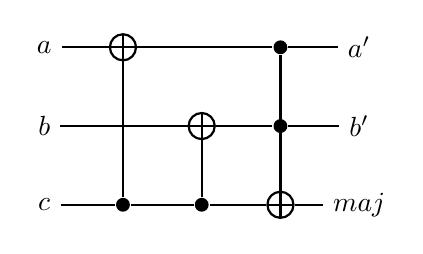
\begin{tikzpicture}[thick]
            %
            % `operator' will only be used by Hadamard (H) gates here.
            % `phase' is used for controlled phase gates (dots).
            % `surround' is used for the background box.
            % `crossx' is used for the cross.
            % `circlewc' is used for the circle with cross box.
            \tikzstyle{operator} = [draw,fill=white,minimum size=1.5em] 
            \tikzstyle{phase} = [fill,shape=circle,minimum size=5pt,inner sep=0pt]
            \tikzstyle{surround} = [fill=blue!10,thick,draw=black,rounded corners=2mm]
            \tikzstyle{circlewc} = [draw,circle,cross,minimum width=0.3 cm]
            \tikzstyle{cross} = [path picture={ 
                \draw[thick,black](path picture bounding box.north) -- (path picture bounding box.south) (path picture bounding box.west) -- (path picture bounding box.east);
                }]
            \tikzstyle{crossx} = [path picture={ 
                \draw[thick,black,inner sep=0pt]
                (path picture bounding box.south east) -- (path picture bounding box.north west) (path picture bounding box.south west) -- (path picture bounding box.north east);
                }]
            % Qubits
            \node at (0,0) (a) {$a$};
            \node at (0,-1) (b) {$b$};
            \node at (0,-2) (c) {$c$};
            %
            % Column 1
            \node[circlewc] (op11) at (1,0) {} edge [-] (a);
            \node[phase] (op31) at (1,-2) {} edge [-] (c);
            \draw[-] (op11) -- (op31);
            %
            % Column 2
            \node[circlewc] (op22) at (2,-1) {} edge [-] (b);
            \node[phase] (op32) at (2,-2) {} edge [-] (op31);
            \draw[-] (op22) -- (op32);
            %
            % Column 4
            \node[phase] (op13) at (3,0) {} edge [-] (op11);
            \node[phase] (op23) at (3,-1) {} edge [-] (op22);
            \node[circlewc] (op33) at (3, -2) {} edge [-] (op32);
            \draw[-] (op13) -- (op33);
            %
            % Column 5
            \node (op14) at (4,0) {$a'$} edge [-] (op13);
            \node (op24) at (4,-1) {$b'$} edge [-] (op23);
            \node (op34) at (4, -2) {$maj$} edge [-] (op33);
        \end{tikzpicture}
    }
    \caption{majority gate (MAJ)}
    \label{fig:MAJ}
\end{figure}
%

To build quantum comparator that outputs whether $A$ is more than $B$ or not. We took Cuccaro adder and modified it using the extension in \citep{Cuccaro2004}. Since we only interest in the highest bit of the adder and we don't care about the sum result. We can build quantum comparator by propagating the carry (or the majority of three qubit) to the most significant bit, put it in the output bit, and reverse the majority step. Figure \ref{fig:compcirc} depicts three bit quantum comparator using this method, output bit at $s_0$.

%
\begin{figure}[t]
    \includegraphics[width=\linewidth]{Figures/cuccaro-comp.png}
    \caption{quantum comparator based on Cuccaro adder}
    \label{fig:compcirc}
\end{figure}
%

Taking controlled-Not gate optimisation method from \citep{Maslov2016}, we can use the same techniques of using relative phase to make relative phase MAJ gate (RMAJ) gate. One version of relative phase Toffoli gate, Margolous gate, is depicted in Figure \ref{fig:rccx}. By replacing Toffoli gate in MAJ gate with Margolous gate, this RMAJ gate will only differ to MAJ on $\ket{011}$ input, which maps $\ket{011}$ to $-\ket{101}$ instead of $\ket{101}$. This phase difference does not pose a problem since our entire circuit does not rely on phase change during the carry ripple process. Also we fix the phase back to its original phase using inverse of RMAJ (iRMAJ) which can be implemented easily by reversing gate order and inverting the gate.
%
\begin{figure}[b]
    \centerline{
        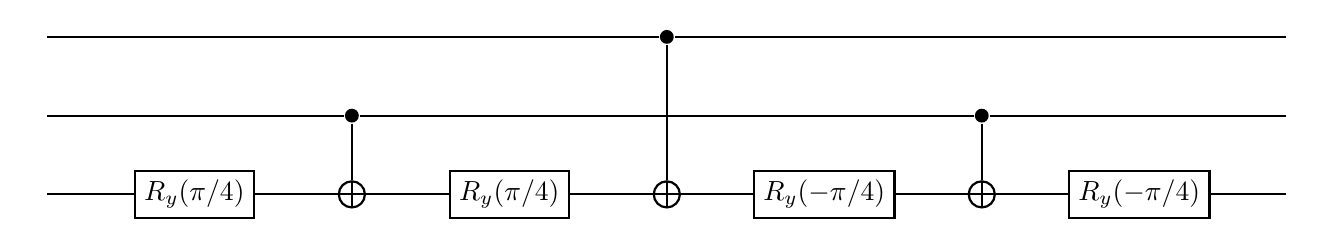
\begin{tikzpicture}[thick]
            %
            % `operator' will only be used by Hadamard (H) gates here.
            % `phase' is used for controlled phase gates (dots).
            % `surround' is used for the background box.
            % `crossx' is used for the cross.
            % `circlewc' is used for the circle with cross box.
            \tikzstyle{operator} = [draw,fill=white,minimum size=1.5em] 
            \tikzstyle{phase} = [fill,shape=circle,minimum size=5pt,inner sep=0pt]
            \tikzstyle{surround} = [fill=blue!10,thick,draw=black,rounded corners=2mm]
            \tikzstyle{circlewc} = [draw,circle,cross,minimum width=0.3 cm]
            \tikzstyle{cross} = [path picture={ 
                \draw[thick,black](path picture bounding box.north) -- (path picture bounding box.south) (path picture bounding box.west) -- (path picture bounding box.east);
                }]
            \tikzstyle{crossx} = [path picture={ 
                \draw[thick,black,inner sep=0pt]
                (path picture bounding box.south east) -- (path picture bounding box.north west) (path picture bounding box.south west) -- (path picture bounding box.north east);
                }]
            % Qubits
            \node at (-1,0) (q1) {};
            \node at (-1,-1) (q2) {};
            \node at (-1,-2) (q3) {};
            %
            % Column 1
            \node[operator] (n31) at (1,-2) {$R_y(\pi/4)$} edge [-] (q3);
            %
            % Column 3
            \node[phase] (n22) at (3,-1) {} edge [-] (q2);
            \node[circlewc] (n32) at (3,-2) {} edge [-] (n31);
            \draw[-] (n22) -- (n32);
            %
            %
            % Column 5
            \node[operator] (n33) at (5,-2) {$R_y(\pi/4)$} edge [-] (n32);
            %
            % Column 7
            \node[phase] (n14) at (7,0) {} edge [-] (q1);
            \node[circlewc] (n34) at (7,-2) {} edge [-] (n33);
            \draw[-] (n14) -- (n34);
            %
            %
            % Column 9
            \node[operator] (n35) at (9,-2) {$R_y(-\pi/4)$} edge [-] (n34);
            %
            % Column 11
            \node[phase] (n26) at (11,-1) {} edge [-] (n22);
            \node[circlewc] (n36) at (11,-2) {} edge [-] (n35);
            \draw[-] (n26) -- (n36);
            %
            %
            % Column 13
            \node[operator] (n37) at (13,-2) {$R_y(-\pi/4)$} edge [-] (n36);
            %
            %
            % Column 15
            \node (n18) at (15,0) {} edge [-] (n14);
            \node (n28) at (15,-1) {} edge [-] (n26);
            \node (n38) at (15, -2) {} edge [-] (n37);
        \end{tikzpicture}
    }
    \caption{Margolous gate}
    \label{fig:rccx}
\end{figure}
%
%
\begin{figure}[b]
    \includegraphics[width=\linewidth]{Figures/rmaj.png}
    \caption{reverse majority gate (RMAJ)}
    \label{fig:rmaj}
\end{figure}
%
% \IncMargin{1em}
\begin{algorithm}[H]
\DontPrintSemicolon
\SetKwData{Left}{left}\SetKwData{This}{this}\SetKwData{Up}{up}
\SetKwFunction{Union}{Union}\SetKwFunction{FindCompress}{FindCompress}
\SetKwInOut{Input}{input}\SetKwInOut{Output}{output}
\Input{$A=a_{n-1}a_{n-2}a_{n-3}\dots a_{0}$, $B=b_{n-1}b_{n-2}b_{n-3}\dots b_{0}$, $z=z$, $c=0$}
\Output{$A=a_{n-1}a_{n-2}a_{n-3}\dots a_{0}$, $B=b_{n-1}b_{n-2}b_{n-3}\dots b_{0}$, $z=z\oplus s_{n}$, $c=0$}
\BlankLine
\For{$i\leftarrow 0$ \KwTo $n-1$}{
    \emph{$b_{i} \leftarrow \sim b_{i}$}\;
}
\emph{$b_{0} \leftarrow MAJ(a_{0}, b_{0}, c)$}\;
\For{$i\leftarrow 1$ \KwTo $n-1$}{
    \emph{$b_{i} \leftarrow MAJ(a_{i}, b_{i}, b_{i-1})$}\;
}
\emph{$z \leftarrow z \oplus b_{n-1} $}\;
\For{$i\leftarrow n-1$ \KwTo $1$}{
    \emph{$b_{i} \leftarrow RMAJ(a_{i}, b_{i}, b_{i-1})$}\;
}
\emph{$b_{0} \leftarrow RMAJ(a_{0}, b_{0}, c)$}\;
\For{$i\leftarrow 0$ \KwTo $n-1$}{
    \emph{$b_{i} \leftarrow \sim b_{i}$}\;
}
\caption{greater than}\label{algo_GT}
\end{algorithm}\DecMargin{3em}
